\section{RPCs}
\label{AppendixF}
The RPCs have been made for the interim report, due to some changes during the project the RPCs have changed a little.
\subsection*{Requirements}
\begin{itemize}
\item Reduction of the stresses in the design during operation and shut-down conditions so that a safety factor of 3 is achieved \cite{safetyfactors}.
\item The stator must be manufacturable with milling \cite{milling} and turning \cite{turning}, standard machining techniques \cite{manufacturingprocess}. Because of this, the wall thickness has to be 0.5 [mm] and the surface roughness has to be $\pm$ 0.0254 [mm].
\item The stator needs to be able to withstand the temperatures shown in Figure \ref{Temperature of the stator}. In this figure, red is 350 $^{\circ}$C, blue 650 $^{\circ}$C and green 150 $^{\circ}$C at shut-down and 750 $^{\circ}$C during operation. 
\end{itemize}

\begin{figure}[h!]
\centering
\begin{minipage}{.5\textwidth}
  \centering
  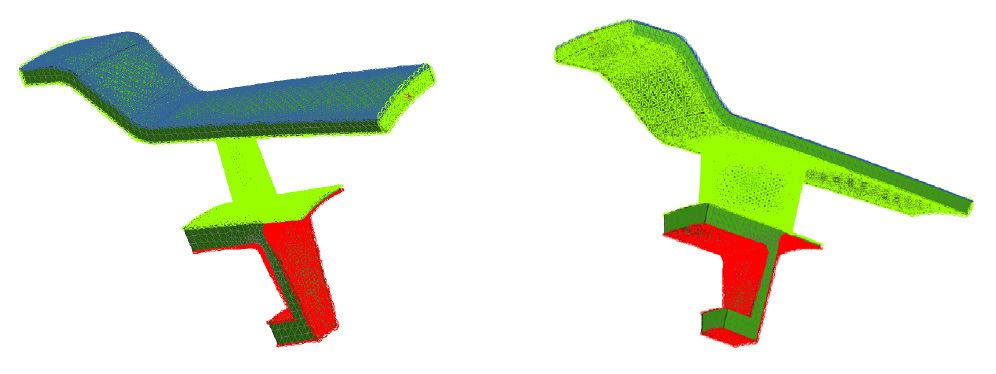
\includegraphics[width=1\linewidth]{Figures/temperature.png}
  \captionof{figure}{Temperature of the stator \cite{COC}}
  \label{Temperature of the stator}
\end{minipage}%
\begin{minipage}{.5\textwidth}
  \centering
  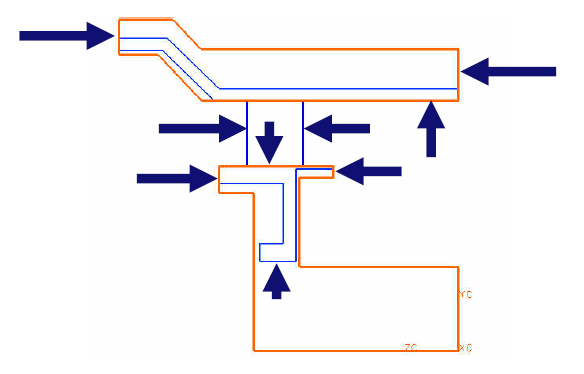
\includegraphics[width=1\linewidth]{Figures/constraints.png}
  \captionof{figure}{Stator with constraints \cite{COC}}
  \label{orange outline}
\end{minipage}
\end{figure}
\subsection*{Preferences}
\begin{itemize}
\item The stator should be made as durable as possible (without changing the performance of the stator)
\end{itemize}

\subsection*{Constraints}
\begin{itemize}
\item The stator blade may not be modified.
\item The stator should retain its functionality: to convert the increased rotational kinetic energy, caused by the blades, into static pressure through diffusion and redirect the flow direction preparing it for the blades of the next stage. 
\item Despite changes on the stator, it should still retain compatible with the other parts.
\item The material Inconel-718-aged (NX libref 45) must be used.
\item Surfaces may not be changed in direction of the arrows and others must remain within the casting (orange outline), shown in Figure \ref{orange outline}.
\end{itemize}
